% ---------------------------------------------------------------------------
% Factor-combination discovery as stochastic threshold group testing
%
% Manuscript source, written to the structure a general-interest methods
% journal expects (abstract, introduction, results, discussion, methods), which
% converts with little work to the alternatives:
%
%   Nature Communications / Cell Systems : as written.
%   PLOS Computational Biology           : add the Author summary (kept below),
%                                          move Methods before Results.
%   Bioinformatics                       : cut to 7 pages by dropping Section
%                                          2.5 and Figure 5.
%
% Build:  pdflatex main && bibtex main && pdflatex main && pdflatex main
% ---------------------------------------------------------------------------
\documentclass[11pt]{article}

\usepackage[utf8]{inputenc}
\usepackage[T1]{fontenc}
\usepackage[margin=1in]{geometry}
\usepackage{graphicx}
\usepackage{booktabs}
\usepackage{amsmath,amssymb}
\usepackage[expansion=false]{microtype}
\usepackage[labelfont=bf,font=small]{caption}
\usepackage[numbers,sort&compress]{natbib}
\usepackage[hidelinks]{hyperref}

\graphicspath{{./}}

\title{\textbf{Factor-combination discovery is stochastic threshold group
testing: a counterfactual replay of the 2006 reprogramming screen}}

\author{Mashal Saleh Alkhalifah\thanks{Institute of Smart Cities, King
Abdulaziz City for Science and Technology (KACST), Riyadh, Saudi Arabia.
Correspondence: \texttt{mkhalifah@kacst.gov.sa}}}

\date{\today}

\begin{document}
\maketitle

\begin{abstract}
\noindent
Finding the few transcription factors that drive a cell-fate conversion is
expensive: every query is a wet-lab assay, and the 2006 screen for the
reprogramming factors consumed a documented 61 under a fixed leave-one-out
protocol. We show that this class of screen is an instance of
\emph{stochastic threshold group testing}, and replay it on an oracle
calibrated to published assay figures. Five results follow.
(1) Information-gain design recovers the hidden recipe in a median of 10
experiments against 61, cheaper in 300 of 300 paired replicates; the same
inference with random pools needs 44, locating the gain in experiment
selection, not inference. (2) An apparent scaling limit, a
classical search overtaking the designer at 48 candidates, is a property of
the proposals rather than the method: changing only which pools may be scored
drops the growth exponent from $n^{1.6}$ to $n^{0.43}$ at 100\%
recovery, where the classical search falls to 83\%. (3) Fixing the recipe
cardinality fails \emph{symmetrically and silently}, at 0.999 confidence
whether the true recipe is smaller or larger; making size latent removes this
for one extra experiment. (4) Audited against two measured perturbation datasets, the
assumed gap response of 0.10 should be 0.77; re-run on that structure the
designer as calibrated recovers 2.5\% of recipes, at mean posterior confidence
0.991 on its failures. (5) That precondition is removable: making the gap
response latent recovers 99.3\%, at 0.4 experiments above an oracle told its
value, and beats a five-experiment calibration pilot on cost and accuracy. The
replay validates the procedure, not the oracle, which was calibrated from the
screen replayed; only (4) tests it against independent data. Results 3--5 are one finding: every assay parameter such a designer fixes is a
silent failure awaiting a system that disagrees, and the remedy is to make it
latent rather than calibrate it better.
\end{abstract}

\section*{Author summary}
\small
When biologists search for the handful of genes that convert one cell type into
another, each guess costs weeks of laboratory work. We asked a counterfactual
question about a famous example: had the 2006 screen for the reprogramming
factors been planned adaptively, how many experiments would it have taken? On a
simulator calibrated to the original paper's numbers, about ten instead of
sixty-one. More useful than that number is where the approach breaks. The
problem turns out to be a known mathematical one --- threshold group testing ---
which supplies both a theoretical yardstick and a classical algorithm as a
competitor. That competitor appeared to win once the candidate gene list passed
about forty, which would have confined the adaptive approach to the regime the
historical screen occupied; tracing the cause showed instead that the adaptive
designer was being offered the wrong experiments to choose among, and supplying
the right ones restores its advantage at every list length we tested. We also
find a failure that matters for anyone deploying these methods: if the number
of genes in the recipe is fixed in advance and that number is wrong, the search
fails while reporting near-certainty, whether the true recipe is larger or
smaller. Finally, we check the model's central assumption against real
measurements, find it wrong in the direction that causes exactly this kind of
confident failure, and then run the method on the corrected landscape: it
recovers the right answer in one run in forty while reporting itself almost
certain. The repair turns out to be the same one: stop fixing the number and
let the search work it out, which restores the method to full accuracy for
less than one extra experiment and beats calibrating it in advance. The
general lesson is that an adaptive method is only as trustworthy as the assay
model it carries, and that anything such a model treats as known in advance is
a confident failure waiting for a biological system that disagrees.
\normalsize

\section{Introduction}

A cell-fate conversion driven by defined factors is, computationally, a
subset-identification problem: of $n$ candidates, an unknown subset $R$ of size
$k$ is sufficient, and the task is to find $R$. What makes it hard is not the
size of the space but the price of a query. Each query is a transduction
experiment with a biological readout, so budgets are counted in tens.

The canonical instance is the screen of \citet{takahashi2006}, extended to human
cells the following year \citep{takahashi2007}. Twenty-four candidates were
selected from the literature; the readout was the number of
drug-resistant colonies surviving Fbx15/G418 selection; and the search followed
a fixed protocol --- each factor alone, the full pool, leave-one-out from the
pool, then leave-one-out from the surviving subset --- consuming $2n + 13 = 61$
experiments at $n = 24$ regardless of what the data said.

Adaptive experimental design \citep{lindley1956, chaloner1995, rainforth2024}
should improve on a protocol fixed in advance, and in perturbation biology
several groups have shown that it does \citep{zhang2023, tosh2025}. What has not been established is
the counterfactual for a specific documented discovery: not predictive accuracy
over an adaptively collected dataset, but the number of wet-lab experiments
needed to reach a known answer under the assay actually used. The 2006 screen
is a good vehicle precisely because its experiment count is in the public
record.

Our second contribution is a reclassification. The colony assay is not generic
combinatorial search: a pool produces colonies efficiently only when it contains
all of $R$, weakly when it contains all but one, and not at all otherwise. In
group-testing language \citep{dorfman1943, aldridge2019}, a test is negative at or below a
lower threshold $l$, positive at or above an upper threshold $u$, and stochastic
in the gap $g = u - l - 1$. This is threshold group testing
\citep{damaschke2006} in its stochastic form \citep{chan2013}, with $u = k$,
$l = k - 2$ and $g = 1$. The reclassification is load-bearing rather than
decorative: it supplies a theoretical yardstick for the achievable test count
and classical algorithms as baselines, and both change the conclusions one would
otherwise draw.

\paragraph{Related work.} Four literatures meet here, and the closest work in
each sits a measurable step away from this one.

\emph{Group testing} supplies the problem class and its bounds, from the
original pooled-screen argument \citep{dorfman1943} through the modern
information-theoretic treatment \citep{aldridge2019}. The variant that matches
this assay is threshold group testing \citep{damaschke2006} in its stochastic
form \citep{chan2013}, and designs for it continue to improve
\citep{bui2024}. Those designs are parameterised by the threshold $u$: it is
given, and the algorithm is built around it. Here $u = |R|$ is exactly what the
experimenter does not know, which is the gap Section~\ref{sec:cardinality}
addresses. Group testing is also being applied to biology right now
\citep{talamanca2026}, but in its disjunctive form --- a pool is positive if it
contains any positive item --- and largely non-adaptively, whereas a
reprogramming pool is positive only if it contains \emph{all} of the recipe.

\emph{Bayesian experimental design} supplies the criterion
\citep{lindley1956, chaloner1995, rainforth2024}. Applied to perturbation
biology, it has been used to choose genetic interventions \citep{zhang2023} and
combination drug screens \citep{tosh2025}, and recent work learns an acquisition
policy amortised over more than a thousand historical CRISPR screens
\citep{edwards2026} or selects gene pairs with a predictive model in the loop
\citep{qin2025}. These are evaluated on hit-recovery or predictive accuracy at a
fixed budget fraction. None asks the counterfactual question of this paper: how
many experiments a documented discovery would have taken, measured against the
count that discovery actually consumed.

\emph{Prediction rather than design} is the third line: ranking reprogramming
factors from expression and network data \citep{rackham2016}, scoring
transcription-factor combinations from single-cell multiomics
\citep{tfcomb2025}, and predicting outcomes of unseen multi-gene perturbations
\citep{roohani2022}. The closest of these even frames its accuracy in
experiment-count terms --- a cocktail ranked fiftieth implies fifty experiments
--- but the ranking is static: it does not condition on results as they arrive,
and the count is a corollary of the ranking rather than a measured search cost.
Such models are nonetheless the natural replacement for the oracle used here,
which is the direction the virtual-cell programme points \citep{bunne2024}.

\emph{Validation of adaptive policies} is the fourth. Held-out evaluations of
selective measurement rules in biological screens have found that the evidence
often fails to justify adopting them over a fixed plan \citep{bi2026}, a
finding that sits naturally beside Section~\ref{sec:stopping}: efficiency and
error detectability pull in opposite directions.

Against that background the contributions of this paper are the counterfactual
against a historical experiment count, the regime boundary against a classical
algorithm, the treatment of an unknown threshold in a threshold-group-testing
assay, and a check of the assay model's central assumption against measured
data.

We state plainly what this study is not. The oracle is a simulator calibrated to
summary figures, not an assay and not a fit to raw data; Section~\ref{sec:real}
is where measured data enters, and it refutes part of the calibration. No claim
about cellular biology follows from any result here.

One inference in particular is unavailable to us, and we flag it because it is
the natural reading of a replay. \textbf{Recovering the Yamanaka factors is not
evidence that the oracle is right.} The oracle was built from the numbers that
screen reported, and the recipe is a truth we planted in it; finding that recipe
therefore tests the search procedure and nothing else. Treating the recovery as
validation of the model would be circular. What the replay measures is the cost
of a search strategy under a documented fitness function, against a published
experiment count --- the same sense in which running a heuristic on a
solved instance measures the heuristic, not the instance. Validation of the
model happens only once in this paper, in Section~\ref{sec:real}, where its
central parameter is compared against measurements it was not fitted to, and
fails.

\section{Results}

\subsection{Cost against the historical record}
\label{sec:main}

\begin{figure}[t]
  \centering
  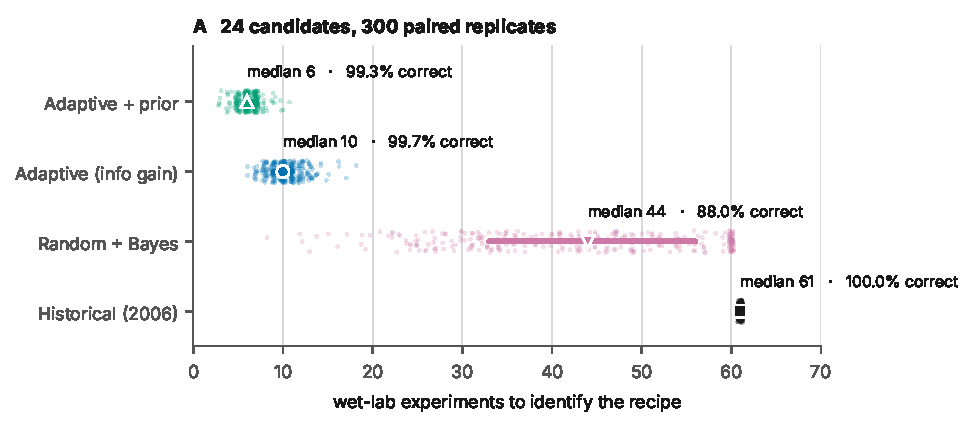
\includegraphics[width=0.86\textwidth]{fig1_main_comparison.pdf}
  \caption{\textbf{Wet-lab cost of four strategies at 24 candidates, 300 paired
  replicates.} Each point is one replicate; bars span the interquartile range,
  markers give medians. The ablation --- the same exact posterior and stopping
  rule with pools drawn at random --- separates the contribution of experiment
  selection from that of inference; its pile-up at 60 is the budget ceiling.}
  \label{fig:main}
\end{figure}

Over 300 replicates (Fig.~\ref{fig:main}), the historical protocol consumes its
fixed 61 experiments; information-gain design needs a median of 10 (95\% CI
[10, 10]; mean 10.3; worst replicate 18) and recovers the exact recipe in
99.7\% of runs; a literature prior reduces this to 6. Paired against the
historical protocol, the adaptive designer is cheaper in 300 of 300 replicates.

Two controls matter more than the headline. The ablation needs a median of 44
experiments and recovers the recipe in 88.0\% of runs; paired, the difference is
32.7 experiments (permutation $p < 10^{-4}$), with the adaptive designer cheaper
in 298 of 300 replicates. The saving comes from informative experiment
selection, not from Bayesian updating. The literature prior buys speed and
nothing else: $-4.1$ experiments ($p < 10^{-4}$) with no detectable accuracy
difference (McNemar $p = 1.0$).

The measured cost should be read against theory rather than against the 2006
protocol alone. For stochastic threshold group testing, test counts of order
$g^2 d \log n$ are achievable \citep{chan2013}; at $g = 1$, $d = 4$, $n = 24$
that is $\approx 13$, consistent with the observed median of 10. The 84\% saving
is therefore not a surprising empirical finding but the expected consequence of
replacing a $\Theta(n)$ protocol with one operating at the model's known order.
That is itself the point: the gap between what the 2006 screen spent and what
was achievable was derivable from theory contemporaneous with it.

\subsection{An apparent regime boundary}
\label{sec:scaling}

\begin{figure}[t]
  \centering
  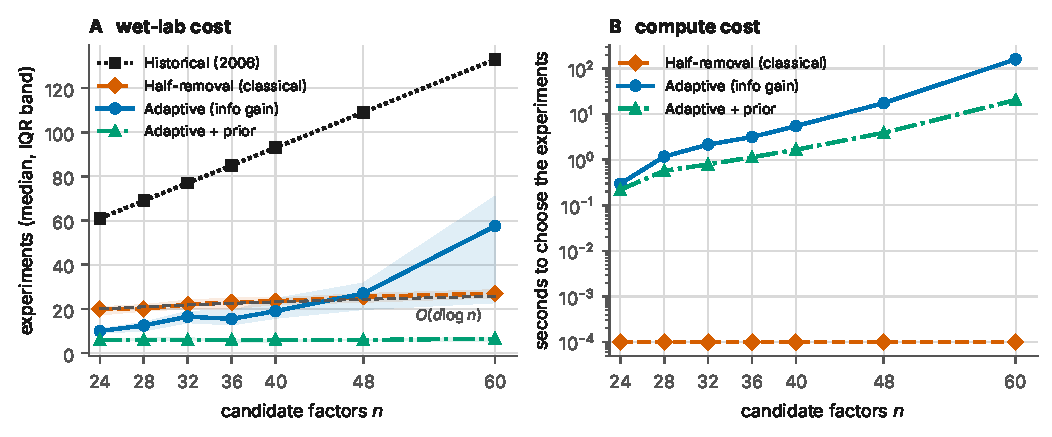
\includegraphics[width=\textwidth]{fig2_scaling.pdf}
  \caption{\textbf{Growth with candidate-list size.} (A) Wet-lab cost, medians
  with interquartile bands, against the $O(d\log n)$ reference curve scaled at
  the smallest list. (B) Compute spent choosing experiments, log scale. The
  classical half-removal search recovers logarithmic growth at negligible
  compute; the Bayesian designer does not, and the two cross at 48 candidates.}
  \label{fig:scaling}
\end{figure}

Yamanaka's 24 candidates were themselves the product of a literature filter, so
a method that works only after such filtering is of limited use.
Figure~\ref{fig:scaling} varies the list from 24 to 60 factors, i.e.\ hypothesis
spaces from $10{,}626$ to $487{,}635$.

The Bayesian designer's wet-lab cost grows as $n^{1.8}$, not logarithmically,
and its advantage over the historical protocol decays from 84\% to 57\%. The
classical half-removal search shows the opposite pattern: twice as expensive at
$n = 24$ (20 versus 10 experiments), it grows as $n^{0.4}$ and the two curves
cross at $n = 48$ (26 versus 27). Because the classical search carries no model
of the assay, this localises the deficiency: not in the inference and not in the
problem, but in proposal generation. Random pools of size 2--12 contain all four
essential factors with probability falling as $n^{-4}$, so as the list grows the
designer evaluates information gain ever more accurately over proposals ever
less likely to be informative. The remedy is a better proposal distribution, and
the classical algorithm is in effect one --- a diagnosis we test directly in
Section~\ref{sec:proposals}, where it proves correct and the boundary
disappears.

Neither method dominates. The classical search pays for its simplicity in
reliability: its success rate falls from 100\% to 83\% as $n$ grows to 60, for a
physical reason rather than an algorithmic one. The pool-size penalty drags a
full 60-factor pool down to about 6 expected colonies, so the positive control
the algorithm starts from approaches the noise floor. The Bayesian designer
holds 100\% at every size because it reasons from the whole count distribution
rather than from one threshold. Compute separates them further: 159~s per run at
$n = 60$ against under a millisecond.

The $k+1$ overlap-class collapse (Section~\ref{sec:methods-inference}) makes the
cost of scoring a proposal independent of posterior concentration, but it
remains linear in the enumerated space, and the number of rounds grows too;
empirically design cost grows as $H^{1.5}$ in the hypothesis count $H$. Exact
enumeration is the binding constraint beyond about 60 candidates. One curve in
Figure~\ref{fig:scaling} must be read with care: the literature-prior variant
appears flat in $n$ only because prior quality is held constant, up-weighting
eight factors regardless of $n$. A longer candidate list implies a less
informative prior, so that curve is an upper bound conditional on prior quality,
not a prediction.

\subsection{The boundary is a property of the proposals, not the method}
\label{sec:proposals}

\begin{figure}[t]
  \centering
  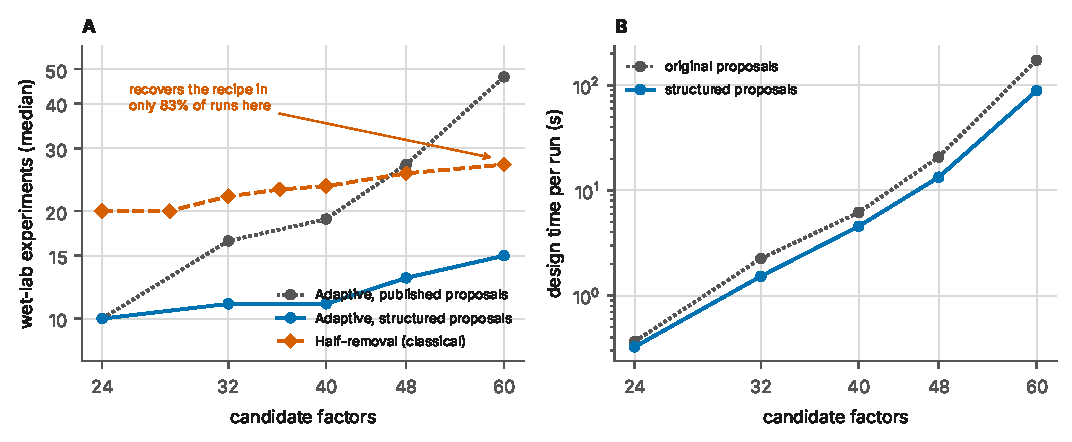
\includegraphics[width=\textwidth]{fig9_proposals.pdf}
  \caption{\textbf{Changing only which pools may be scored.} (A) Median
  wet-lab cost against candidate-list size for the published proposal
  generator, the structured one, and the classical half-removal search of
  Section~\ref{sec:scaling}. The scoring rule, posterior, oracle, recipes and
  seeds are identical across the two adaptive curves, as is the number of pools
  scored per round. (B) The design-time price of the change, which is negative:
  the structured proposals need fewer rounds than their larger pools cost.}
  \label{fig:proposals}
\end{figure}

Section~\ref{sec:scaling} attributed the adaptive designer's poor scaling to its
proposal distribution rather than to its inference. That attribution was an
interpretation of a null result and deserved a direct test, since a method's
authors are poorly placed to decide that its deficiency is the benign kind.

We therefore constructed a second proposal generator and changed nothing else.
It adds the three families the original lacked. \emph{Removal pools}: the
factors carrying appreciable posterior mass, less a random half, quarter or
eighth of them --- precisely the queries by which half-removal halves its live
set, and absent from the original proposals at every list length.
\emph{Complements of ranked prefixes}: a prefix of the marginal ranking asks
whether the recipe lies in the top $k$, and its complement asks the same
question from the side that is more informative when the answer is no.
\emph{Scale-aware random pools}: sizes drawn log-uniformly between the recipe
size and the full candidate set, rather than from a fixed window of 2--12.
Both generators return the same number of pools per round, so no difference can
be bought with a wider search.

The diagnosis holds (Fig.~\ref{fig:proposals}). The growth exponent falls from
$n^{1.61}$ to $n^{0.43}$, against $n^{0.36}$ for the classical search, and the
median cost at 60 candidates falls from 48 experiments to 15 --- below the
classical algorithm's 27 rather than above it. The saving is zero at 24
candidates (0.6 experiments, $p = 0.29$), where the original window already
covered a usable fraction of the space, and grows monotonically with list
length: 5.5 at 32, 8.6 at 40, 19.7 at 48 and 34.2 at 60 experiments per run,
all paired on identical recipes and seeds, all $p < 10^{-3}$. Recovery remains
100\% at every size, where the classical search declines to 83\% at 60 for the
physical reason given above.

Two qualifications. The comparison is confined to the hypothesis spaces exact
enumeration can hold, so it does not show that the Bayesian designer scales
indefinitely; the compute wall of Section~\ref{sec:scaling} is untouched, and
remains the binding constraint past about 60 candidates. And the structured
generator was designed after seeing the failure it repairs, which makes it an
explanation of that failure rather than an independent prediction. What the
experiment establishes is narrower and sufficient: the regime boundary we
reported was contingent on an implementation choice, not a property of
information-gain design, and should not be cited as the latter.

\subsection{Model error: absent signal versus wrong signal}
\label{sec:calibration}

\begin{figure}[t]
  \centering
  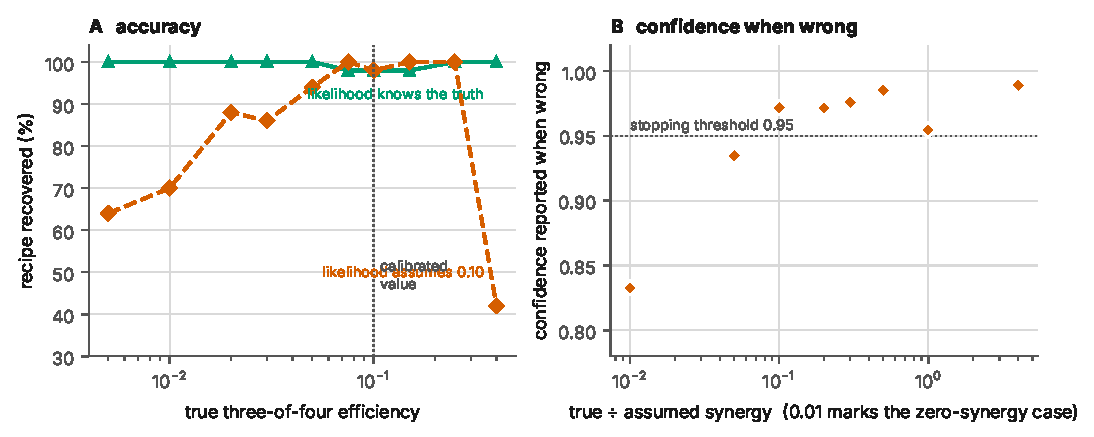
\includegraphics[width=\textwidth]{fig3_calibration.pdf}
  \caption{\textbf{Gap response and calibration error.} (A) Recovery rate as the
  true three-of-four efficiency $\rho$ varies, with the likelihood either
  informed of it or holding the calibrated 0.10. (B) Confidence reported in runs
  that returned a wrong recipe, against the ratio of true to assumed $\rho$ (the
  leftmost point is the zero-gap case).}
  \label{fig:calibration}
\end{figure}

The graded three-of-four signal is the gap response of the threshold model, and
it is natural to suppose the search depends on it. Separating the signal's
presence from the searcher's belief about it shows otherwise
(Fig.~\ref{fig:calibration}A). With the gap response removed entirely
($\rho = 0$) and the likelihood informed of this, the recipe is still recovered
in 100\% of runs at a median of 22 experiments: the search degenerates to pure
group testing, pays a factor of 2.2 for the lost gradient, and remains 64\%
cheaper than the historical protocol. The same oracle with a searcher that keeps
believing $\rho = 0.10$ succeeds in 52\% of runs. Absence of graded synergy is a
calibration error, not a structural barrier.

What binds is the magnitude of the error, asymmetrically. Under-estimating the
gap response fivefold still recovers the recipe in 70\% of runs, while
over-estimating it fourfold drops recovery to 42\% --- and reports confidence
0.989 while doing so. Conservative calibration is the safer error direction,
which matters because the gap response is exactly the quantity a pilot
experiment estimates poorly.

\subsection{Assumed cardinality: a symmetric, silent failure}
\label{sec:cardinality}

\begin{figure}[t]
  \centering
  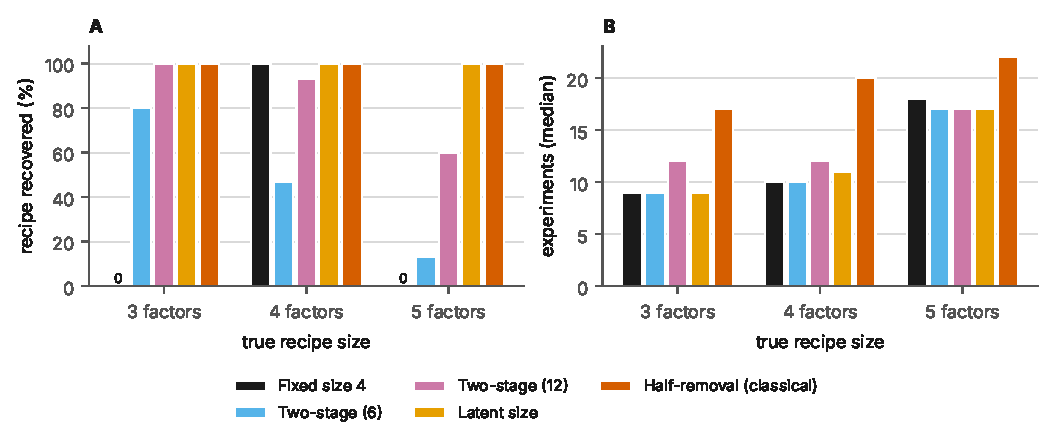
\includegraphics[width=\textwidth]{fig4_cardinality.pdf}
  \caption{\textbf{Unknown recipe size, several treatments, three truths.}
  (A) Exact-recipe recovery. (B) Cost. Fixing the size at four fails completely
  when the truth is three or five; estimating the size in a first stage and
  committing to it inherits the failure whenever the estimate is wrong; carrying
  size as a latent variable, or dispensing with a size representation
  altogether, does not.}
  \label{fig:cardinality}
\end{figure}

Every result above assumes the searcher knows $k = 4$. Relaxing that assumption
exposes the method's one genuinely structural failure
(Fig.~\ref{fig:cardinality}). A designer fixed at four factors recovers a
three-factor recipe in 0\% of runs and a five-factor recipe in 0\% of runs, and
in both cases reports a mean posterior confidence at or above 0.99 on the wrong
answer. The failure is symmetric: searching for more factors than exist is as
fatal as searching for fewer, because the fixed designer appends a spurious
factor to a correct core and then concludes. This is not a failure of the data
but of a hypothesis space that cannot represent the truth, and the posterior is
confident precisely because every hypothesis it can represent is wrong by the
same margin.

Treating cardinality as latent removes it. Recovery is 100\% at true sizes
three, four and five; the correct size carries posterior mass 0.995 or above in
all three cases; and the premium on the four-factor case the fixed designer was
built for is $+0.9$ experiments (paired $p = 0.0036$). The latent treatment also
returns a diagnostic the fixed designer cannot produce even in principle: a
posterior over recipe size, which is what would tell an experimenter that their
assumed cardinality was wrong.

Two comparators place this result. The classical answer to unknown $|R|$ is to
estimate the count in a first stage and then commit to it \citep{bshouty2018}.
That baseline inherits the failure whenever the first stage errs, and it errs
often: with a six-experiment first stage it commits to the wrong size in 53\% of
four-factor runs and 87\% of five-factor runs, recovering the recipe in 47\% and
13\% of them; doubling the first stage to twelve experiments reduces the wrong
commitments to 7\% and 40\%, for 93\% and 60\% recovery, at a cost of
$+1.7$ experiments on the four-factor case ($p = 0.005$). Carrying the size
posterior throughout instead of committing to it is thus not redundant
machinery: it is what converts a 60\% method into a 100\% one at no measurable
premium ($+0.5$ experiments, $p = 0.53$). The model-free half-removal search
sidesteps the question entirely, since it never represents a size, and recovers
all three sizes without modification --- for $+9.7$ experiments
($p < 10^{-4}$), roughly double. Cardinality is therefore a liability of the
parametric approach specifically, not of the problem.

\subsection{The stopping rule, and a trade-off between efficiency and
detectability}
\label{sec:stopping}

\begin{figure}[t]
  \centering
  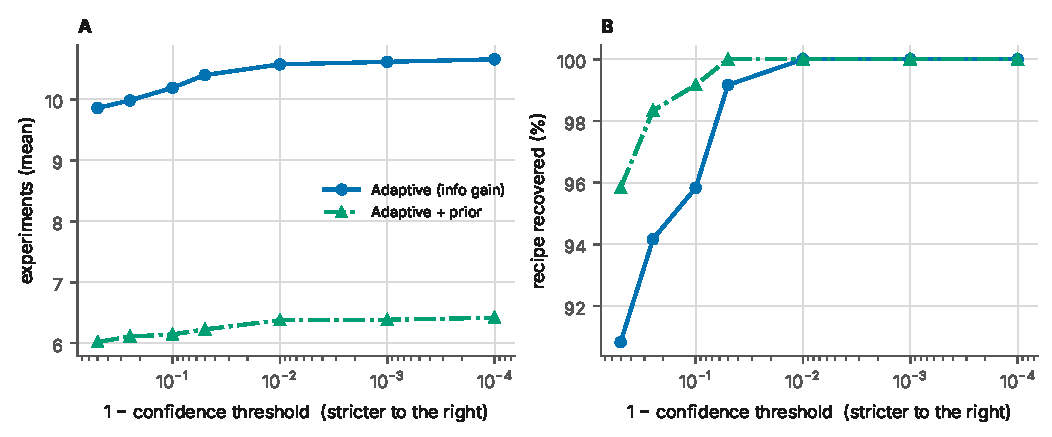
\includegraphics[width=\textwidth]{fig5_stopping_rule.pdf}
  \caption{\textbf{The price of certainty.} (A) Mean experiments and (B)
  recovery rate as the stopping threshold tightens from 0.50 to 0.9999. Cost is
  nearly flat while accuracy improves, because posterior confidence jumps at the
  decisive experiment rather than climbing gradually.}
  \label{fig:stopping}
\end{figure}

A Bayesian stopping rule is usable only if its confidence means what it says,
since in a real campaign there is nothing to check it against. Sweeping the
threshold from 0.50 to 0.9999 (Fig.~\ref{fig:stopping}), the stated confidence
never exceeds the observed recovery rate by more than its Wilson interval
permits (largest discrepancy $+0.025$), and tightening by four orders of
magnitude costs 0.8 experiments on average while never moving the median. The
practical recommendation is to run at 0.999 or tighter.

That flatness is the mechanism behind a pattern visible throughout. Confidence
does not accumulate gradually; it jumps at the decisive experiment, so there is
no intermediate regime in which the searcher can report that it is not sure yet.
When the model is wrong, high confidence therefore arrives just as promptly on
the wrong answer: the adaptive designer's mean confidence when wrong is 0.955
against 0.423 for the random-pool ablation; an over-estimated gap response fails
at 0.989; a cardinality mismatch fails at 0.999. The designer is well calibrated
\emph{inside its model}, and that does not protect it when the model is wrong.
Efficient experiment selection improves cost and degrades the detectability of
model error at the same time, because a procedure that gathers consistent
evidence quickly gathers it quickly for a wrong hypothesis too.

\subsection{The gap assumption against measured data}
\label{sec:real}

\begin{figure}[t]
  \centering
  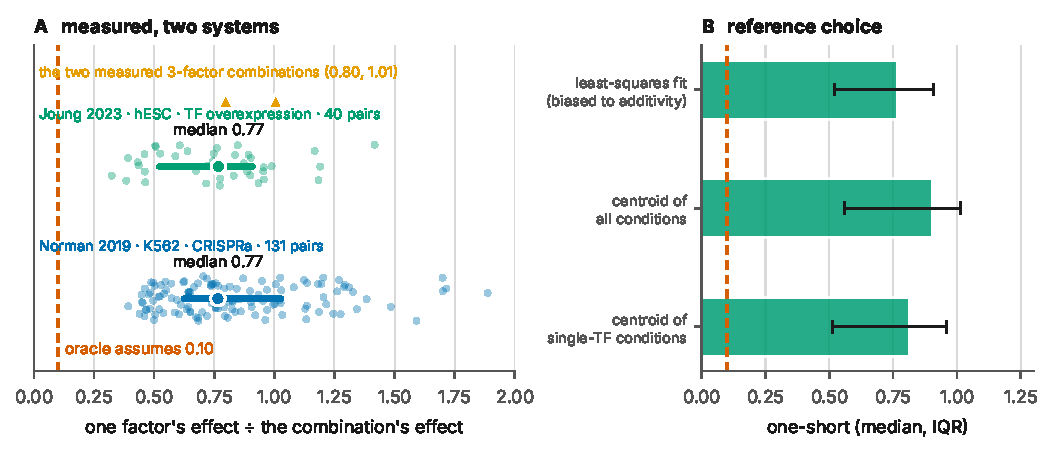
\includegraphics[width=\textwidth]{fig6_real_data.pdf}
  \caption{\textbf{What one factor of a measured combination reproduces.}
  (A) The ratio $\lVert\delta_{\text{one short}}\rVert /
  \lVert\delta_{\text{combination}}\rVert$ for 131 gene pairs in K562
  \citep{norman2019} and 40 transcription-factor pairs in human embryonic stem
  cells \citep{joung2023}, with the two measured three-factor combinations
  marked. The oracle assumes 0.10. (B) The hESC subset has no unperturbed
  control, so three references are reported; the conclusion does not depend on
  the choice.}
  \label{fig:real}
\end{figure}

Every result above is conditional on gap structure of the assumed shape
existing. Single-cell perturbation screens now cover enough combinations to
check it directly \citep{replogle2022, peidli2024}, and two of them carry the
pairs and singles the measurement needs. For a perturbation $p$ with
pseudobulk profile $x_p$ and reference $x_0$, write
$\delta_p = x_p - x_0$; for each combination whose one-short constituents were
also profiled, we measure
\begin{equation}
  \text{one-short} =
  \frac{\max_{c}\ \lVert \delta_c \rVert}{\lVert \delta_{\text{combination}} \rVert},
  \label{eq:oneshort}
\end{equation}
the empirical analogue of $\rho$, whose calibrated value is 0.10.

In \citet{norman2019} --- K562, CRISPRa, 131 pairs with both singles measured
--- the median is \textbf{0.77} (IQR 0.62--1.03), and \textbf{no pair of the 131}
falls below 0.20. In the combinatorial subset of \citet{joung2023} --- human
embryonic stem cells, transcription-factor overexpression, 40 TF--TF pairs ---
the median is \textbf{0.77} (IQR 0.52--0.91) under a reference fitted by least
squares, 0.91 and 0.82 under two alternative references, with no pair below 0.20
under any of them (Fig.~\ref{fig:real}B). The two measured three-factor
combinations give 0.80 and 1.01.

The result is not an artefact of measuring effect size by a Euclidean norm.
Repeating the Norman analysis with threshold-like functionals --- the number of
genes moving more than 0.25 or 0.5 in log space --- lowers the median to 0.48
and 0.50 and raises the fraction below 0.20 to 25\% and 22\%, but no functional
produces a median near 0.10.

Two further observations. First, departures from additivity are common but
modest in magnitude: in Norman the median ratio of the pair's effect to the sum
of its singles is 0.91, with 47\% of pairs sub-additive and 27\% super-additive,
and only 28\% of pairs have an additivity residual exceeding its own sampling
noise, estimated by regressing squared residuals on
$1/n_{AB} + 1/n_A + 1/n_B$. Second, the two systems differ in \emph{where} the
interaction lives: the median $R^2$ of a pair on its two singles is 0.86 in
K562 but 0.64 in hESCs, so combinations in the stem-cell system leave the plane
spanned by their constituents more, while their magnitudes remain near-additive.

The implication is specific. Our calibrated $\rho = 0.10$ is five- to eightfold
sharper than measurement supports, and Section~\ref{sec:calibration} shows that
over-estimating the gap response is precisely the direction in which the
designer fails silently. A designer calibrated as ours is would therefore be
expected to fail confidently on these systems, while the same designer informed
of the true $\rho$ succeeds in 98--100\% of runs at every value tested,
including $\rho = 0$. The gap response must be estimated, not assumed.

The constructive reading is that the oracle should be replaced rather than
recalibrated: a predictive model fitted to measured perturbation outcomes
\citep{roohani2022}, or the broader virtual-cell programme
\citep{bunne2024}, would supply a gap response estimated from data rather than
assumed, and the designer would inherit whatever accuracy that model has. The
experiments above then become the specification for how accurate it must be:
within a factor of two on the gap response, and honest about recipe size.

One boundary deserves emphasis. Both datasets read out the transcriptome, while
the 2006 assay reads out a rare discrete phenotype --- a colony forms or does
not --- which is a thresholded functional of cell state and may well be far
sharper than transcriptome displacement. The audit therefore refutes the
assumption for expression-level objectives and constrains, rather than settles,
the phenotype case. Settling it requires a combinatorial screen with a
phenotypic readout, which to our knowledge does not exist at the scale needed.

\subsection{The designer run on the measured gap structure}
\label{sec:measured-gap}

\begin{figure}[t]
  \centering
  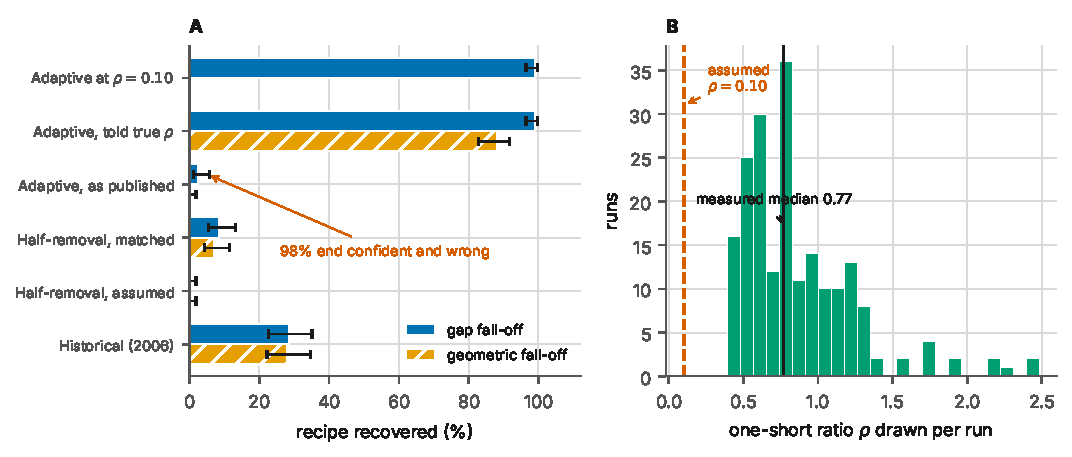
\includegraphics[width=\textwidth]{fig7_measured_gap.pdf}
  \caption{\textbf{Recovery when the gap response is drawn from measurement
  rather than assumed.} (A) Recipe recovered over 200 paired runs per arm, with
  Wilson intervals, under both fall-off shapes. The designer carrying this
  study's published calibration recovers the recipe in 2.5\% of runs and stops
  on its own confidence rule in almost all of the failures. Told the true
  $\rho$, the same designer returns to 99\%. (B) The distribution of $\rho$
  drawn per run, against the value the oracle assumes.}
  \label{fig:measuredgap}
\end{figure}

Section~\ref{sec:real} established that $\rho = 0.10$ is far sharper than
measurement supports, and inferred from Section~\ref{sec:calibration} that a
designer calibrated this way \emph{would be expected} to fail confidently. An
inference of that weight should be measured rather than inferred. We therefore
re-ran the search with $\rho$ drawn per replicate from the 131 measured Norman
ratios and held fixed across arms, so that every method meets the same
landscape (Fig.~\ref{fig:measuredgap}).

The expectation is confirmed, and more sharply than anticipated. Under the gap
fall-off the designer as published recovers the recipe in \textbf{2.5\%} of 200
runs (95\% Wilson interval 1--6\%) against 99.0\% for the same designer informed
of $\rho$ (exact McNemar $p < 10^{-4}$). The failures are not budget
exhaustions: no run reached the cap, the median cost was 9 experiments against
10 for the correctly calibrated reference, and the mean posterior confidence on
runs that ended \emph{wrong} was \textbf{0.991}. The practitioner receives a
four-factor recipe, a tight posterior and no indication of error.

Three consequences follow. First, the fault is in the calibration rather than
the inference: the matched designer costs 12 experiments against 10 at the
assumed $\rho$, so the headline saving survives the realistic landscape
\emph{conditional on knowing} $\rho$. Estimating the gap response is therefore
not a refinement but a precondition, and the natural construction --- carrying
$\rho$ as a latent parameter updated alongside the recipe --- is the obvious
next step rather than an optional one.

Second, the classical algorithm is not a fallback. Half-removal recovers the
recipe in 0.0\% of runs with its assumed threshold and 8.5\% with the threshold
rebuilt at the true $\rho$: when a pool one factor short yields 80\% of a
complete one, no positivity threshold separates them, and being told the truth
does not help because the information is not in the readout. The 2006 protocol
reaches 28.5\%, worse than the matched designer by a wide margin but without a
confidence claim to be wrong about --- it fails audibly.

Third, the conclusion is not an artefact of the sharp fall-off. Under a
geometric shape, where efficiency decays as $\rho$ per missing factor rather
than vanishing beyond one, the published designer recovers nothing at all
(0/200) while the matched designer reaches 88.0\% at a median of 16 experiments
and a mean of 35. Pair measurements constrain the one-short step and say nothing
about what lies beyond it, so both shapes are reported.

\subsection{Discovery against measured data, with no simulator}
\label{sec:retrospective}

\begin{figure}[t]
  \centering
  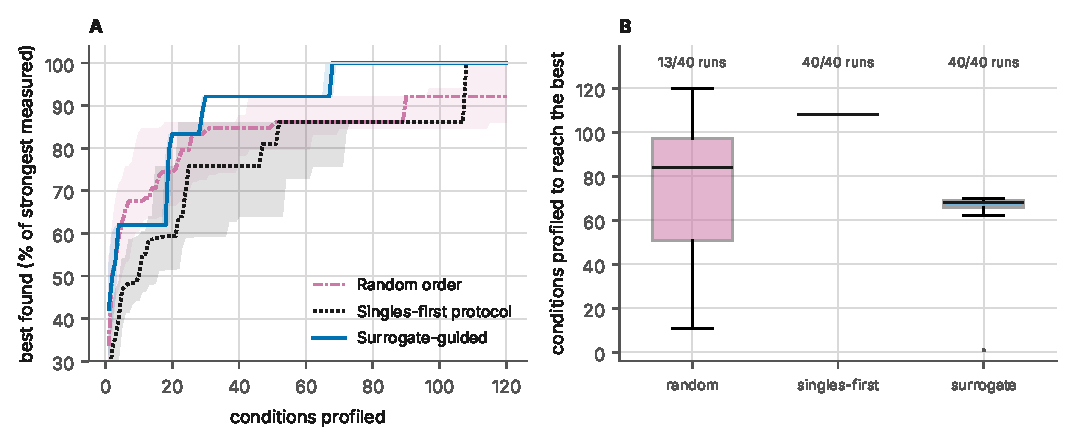
\includegraphics[width=\textwidth]{fig8_retrospective.pdf}
  \caption{\textbf{Sequential discovery where every query returns a
  measurement.} (A) Best condition found so far as a fraction of the strongest
  measured combination, median over 40 replicates with interquartile band. (B)
  Conditions profiled before reaching that combination; the annotation gives
  how many replicates reached it at all, without which the box is not
  comparable.}
  \label{fig:retrospective}
\end{figure}

Experiment~\ref{sec:measured-gap} grounds one parameter of the oracle in
measurement, but still queries a simulator. The strongest available test removes
it. We built an oracle over \citet{norman2019} that answers only for conditions
the authors actually profiled --- 105 singles, 131 pairs and one control ---
returning the magnitude of the measured pseudobulk shift against control,
perturbed by the dataset's own disagreement across two random halves of the gene
panel (median relative discrepancy 0.049). A condition that was not profiled
raises an error rather than being interpolated, since an interpolated answer
would reinstate the simulation the construction exists to remove.

That restriction changes the task. With no pools beyond pairs there is nothing
to design, so this is sequential discovery within a measured library rather than
threshold group testing: find the strongest combination while profiling as few
conditions as possible. It tests the half of the claim that survives --- that
choosing the next experiment from a model beats choosing it by protocol.

The strongest measured combination is \texttt{CEBPA+JUN}. A surrogate fitting
pair response on its constituents' measured singles, queried by
upper-confidence score, reaches it in a median of 68 conditions in 40 of 40
replicates, against 108 for a singles-first protocol and 84 for random order,
which reached it at all in only 13 of 40. At a budget of 20 conditions the
surrogate attains 83\% of the target against 59\% for the protocol (paired
permutation, $p < 10^{-4}$; Fig.~\ref{fig:retrospective}).

The singles-first row should be read as biology before method. A measured
one-short ratio of 0.77 is precisely what makes ``profile the singles, then the
pairs built from the best of them'' nearly sufficient on this landscape. The
simulated assay, in which a single factor yields nothing at all, is the
\emph{easier} of the two problems rather than the harder one --- a point that
the simulation-only version of this study could not have reached.

\subsection{Inferring the gap response rather than assuming it}
\label{sec:latent-gap}

\begin{figure}[t]
  \centering
  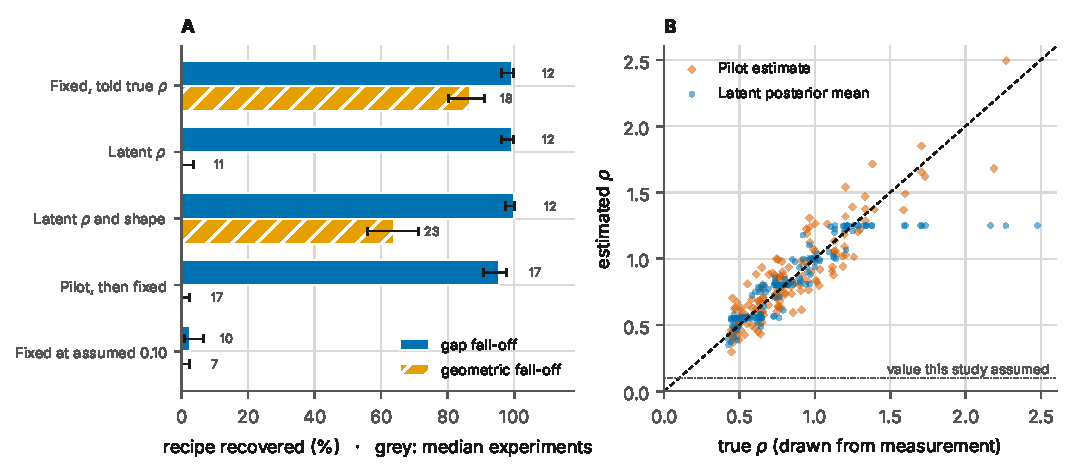
\includegraphics[width=\textwidth]{fig10_latent_gap.pdf}
  \caption{\textbf{Two ways to stop assuming $\rho$.} (A) Recipe recovered
  over 150 paired runs per arm with Wilson intervals, under both true fall-off
  shapes; the grey number beside each bar is that arm's median experiment
  count, since an arm is only cheap if it is also right. The pilot's five
  calibration experiments are counted inside its total. (B) Estimated against
  true $\rho$ for the pilot and for the latent posterior's mean, under the gap
  shape, with the identity line. The latent estimates flatten at 1.25 because
  that is the top of the grid; the pilot has no ceiling but is noisier
  throughout, and both are far from the 0.10 this study assumed.}
  \label{fig:latentgap}
\end{figure}

Section~\ref{sec:measured-gap} leaves $\rho$ as something that must be
obtained rather than assumed. A laboratory would obtain it by calibrating
first: run a recipe already known to work and each of its one-short pools,
take the ratio, then fix $\rho$ and search. The alternative is to carry $\rho$
in the posterior and let the search inform it. Which is cheaper is not obvious
--- the pilot spends whole experiments up front and ends in a point estimate
with its own Poisson error, while joint inference spends part of every
experiment's evidence on a parameter nobody asked about.

The joint posterior is the fixed-size designer with one more index. The
colony distribution depends on a hypothesis and an assay model only through
the pair $(\lvert S \cap h\rvert, m)$, so the five overlap classes become
$5 \times \lvert \mathcal{M} \rvert$ classes and the cost of scoring a
proposal again does not depend on how concentrated the posterior is. We
discretise $\rho$ on nine points spanning the assumed 0.10, the measured range
and the sub-additive region above 1, and stop on the \emph{recipe} marginal
with $\rho$ integrated out, since a designer that waited to pin down a
nuisance parameter would be answering the wrong question. All arms use the
structured proposals of Section~\ref{sec:proposals}, so the generator is not a
confound.

Under the gap fall-off the result is clean (Fig.~\ref{fig:latentgap}). Latent
$\rho$ recovers the recipe in \textbf{99.3\%} of runs at a median of 12
experiments --- indistinguishable from the oracle arm told the true value
(99.3\%, median 12), at a cost of 0.4 experiments on the paired mean. Against
the pilot it is both cheaper and more accurate: 4.7 fewer experiments
($p < 10^{-4}$) at 99.3\% against 95.3\%. Making the shape latent as well
costs nothing measurable and recovers 100\% of recipes. The practical
recommendation is therefore the stronger of the two available: $\rho$ need not
be calibrated in advance at all, and a designer that infers it is no more
expensive than one handed the answer.

The geometric fall-off is where the result stops, and the way it stops is
informative. Latent $\rho$ with the shape still fixed recovers
\textbf{0.7\%} --- no better than the uncalibrated designer. The pilot
recovers \textbf{0\%}, and necessarily so: a pilot measures the one-short step
and is structurally blind to what lies beyond it, so no number it returns can
repair a wrong shape. Only the arm that treats the shape as unknown recovers
anything, at 64.0\% and a median of 23 experiments, against 86.7\% for an
oracle told both shape and $\rho$. That arm identifies the shape essentially
perfectly --- posterior mass on the true shape above 0.9 in 100\% of runs ---
so what limits it is not identifying the model but searching the flat
landscape the model describes, which Section~\ref{sec:measured-gap} already
showed to be hard even with full knowledge. It also fails silently in 18\% of
runs, which is worse than any arm under the gap shape.

The inferred $\rho$ is accurate where the shape is right and biased where it
is not: median absolute error 0.06 against a grid spacing of 0.20--0.25 under
the gap shape, with the 90\% credible interval over grid cells covering the
true value in 86\% of runs --- close to nominal, and a little under it, which
is the expected price of a discrete grid. Under a misspecified shape the same
interval covers in 36\% of runs, so the $\rho$ posterior reports the miss
rather than concealing it.

Two things follow. The parameter this study got wrong is now inferable at no
cost, which removes the precondition of Section~\ref{sec:measured-gap}. But
the broader lesson of that section survives intact: the fix generalises only
as far as the model class does, and a designer that fixes the fall-off
\emph{shape} inherits exactly the failure that fixing $\rho$ produced.
Measured pair data cannot distinguish the shapes, so this is not a gap we can
close with the data in hand; it is the next measurement someone has to make.

\section{Discussion}

Five conclusions survive the controls, and they are narrower than the headline
saving.

The saving is real but unsurprising once the problem is named. Recognising the
colony assay as stochastic threshold group testing with $g = 1$ supplies the
achievable order, $O(g^2 d\log n)$, and the observation that the 2006 protocol
operated at $\Theta(n)$. The contribution is not the adaptive designer but the
quantification: how much of that theoretical gap is realisable under the assay's
noise, with the historical count as the reference.

The Bayesian apparatus does earn its place, but the reason is not the one we
first reported. Measured against a classical conjunctive search it appeared to
lose beyond 48 candidates; giving it the classical algorithm's own queries to
score removes the crossing entirely and leaves it at a third of the cost and a
higher recovery rate at every list length tested
(Section~\ref{sec:proposals}). The episode is worth stating plainly, because
the first version of this analysis would have been published as a regime
claim and the regime was an artefact. What survives is a compute boundary
rather than a statistical one: the design step still costs 89~s per run at 60
candidates against under a millisecond for the classical search, and exact
enumeration remains the binding constraint.

For deployment, the cardinality result is the most actionable: a parametric
designer that fixes recipe size fails silently and symmetrically, the standard
two-stage remedy inherits the failure, and latent-cardinality inference removes
it for about one extra experiment while supplying a size posterior that makes
the error visible. Given the general pattern that efficient design suppresses
the signature of model error, cheap diagnostics of this kind are not optional
extras.

Finally, the real-data audit turns the study's main caveat into a result, and
then into a verdict on the study's own artefact. The assumption that a one-short
pool yields a tenth of the full response is not supported in either measured
system; the measured value is close to 0.8. Running the designer on that
structure rather than reasoning about it (Section~\ref{sec:measured-gap}) gives
2.5\% recovery at a mean posterior confidence of 0.991 on the failures. The
operational rule follows without hedging: measure the gap response in a pilot,
calibrate conservatively, and treat a designer that has not done so as
untrustworthy regardless of what its posterior reports --- including the one
distributed with this paper, which should be run with $\rho$ estimated and not
with the value we calibrated.

Section~\ref{sec:latent-gap} then removes that precondition rather than
leaving it as advice. Carrying $\rho$ in the posterior costs 0.4 experiments
against an oracle told its value, recovers 99.3\% of recipes where the shipped
calibration recovers 2.7\%, and beats a five-experiment pilot on both cost and
accuracy --- so the operational rule simplifies to: do not fix $\rho$, infer
it. The same construction extended to the fall-off shape recovers the shape
with near-certainty, and the arms that fix the shape fail under it exactly as
the arms that fixed $\rho$ failed before. The pattern is the same one three
times over, and it is the paper's most portable finding: \emph{every
parameter this family of designers fixes is a silent failure waiting for a
system that disagrees, and the remedy each time is to make it latent rather
than to calibrate it better.}

\paragraph{What these experiments specify.} Read together, the results are less
a study of one historical screen than a specification for the evaluator that any
such search runs inside. A search procedure consumes an evaluator, and the
questions this paper answers are the ones an evaluator must satisfy before
searching inside it pays: its gap response must be accurate to within about a
factor of two, with under-estimation the safer error
(Section~\ref{sec:calibration}); it must expose uncertainty over structure, not
only a score, because a model that cannot represent the right recipe size fails
silently at 0.999 confidence (Section~\ref{sec:cardinality}); and its stopping
confidence is trustworthy only to the extent its own model is
(Section~\ref{sec:stopping}). Those are testable requirements, and they apply to
a learned model of cell state as much as to the calibrated oracle used here.

The measured data adds a fourth requirement and relaxes one assumption. An
evaluator fitted to expression data will present a graded, near-additive
landscape rather than the sharp threshold the 2006 assay suggests
(Section~\ref{sec:real}), which is easier to search, not harder --- but it also
means the gap response has to be estimated from a pilot rather than inherited
from a published figure.

\paragraph{Where the method ends and another begins.} The scaling result marks
a boundary that matters beyond this benchmark, though not the boundary we
first drew. Exact enumeration over hypotheses is what makes the posterior cheap
and it is also what fails: at 60 candidates the design step costs 89~s per run
even with the structured proposals, and the hypothesis count grows as $n^4$. A
reprogramming search over the roughly 1{,}600 human transcription factors is
three orders of magnitude past that, so the approach used here cannot be
carried to it by tuning. Section~\ref{sec:proposals} is suggestive about what
replaces it: the single change that recovered logarithmic-order growth was to
generate proposals from the current posterior's structure rather than draw them
at random, which is what population-based search does by construction --- a set
of candidates derived from the currently promising ones. The natural successor
is therefore a search whose proposals are generated, whose posterior is
approximate rather than enumerated, and whose evaluator is a learned model,
with the requirements above as its acceptance criteria.

\paragraph{Next steps.} Four follow from the results, in order of what each
would settle. First, replace the calibrated oracle with a retrospective one
built directly from measured combinatorial data, turning every count reported
here from a property of a model into a measurement. Second, rebuild the
proposal distribution along the lines the classical comparator suggests and
test whether logarithmic scaling is recovered, which is the difference between
diagnosing the defect and repairing it. Third, make the gap response a latent
parameter estimated during the search rather than a fixed constant, which the
real-data audit shows is the assumption most likely to be wrong in deployment.
Fourth, and most open: the threshold-group-testing literature parameterises its
designs by a \emph{known} threshold, while the quantity an experimenter lacks is
exactly that threshold. Bounds for threshold group testing with unknown $u$
would place the cardinality result of Section~\ref{sec:cardinality} on a
theoretical footing rather than an empirical one.

\paragraph{Limitations.} The oracle is a simulator calibrated to published
summary figures, so its numbers are properties of a stated model; the design of
the comparisons, not the realism of the oracle, carries the conclusions. The
audit datasets read out expression rather than a rare phenotype, which is the
readout the historical assay used; the evaluator-quality lesson of
\citet{okita2007}, where a better selection marker changed which colonies counted
as success, is the biological form of the same concern. The historical protocol is
reconstructed from
the paper's description rather than laboratory records. The latent-cardinality
designer widens its assumption to sizes 3--6 rather than eliminating it, so a
seven-factor truth would reproduce the original failure. Exact enumeration
limits the approach to candidate lists of order $10^2$, which excludes the
genome-scale setting where a reprogramming screen would benefit most.

\section{Methods}
\label{sec:methods}

\subsection{Oracle}

A hidden essential set $R \subseteq \{1,\dots,n\}$, $|R| = k$, is drawn
uniformly. For a transduced pool $S$, the colony count is a Poisson draw,
\begin{equation}
  y(S) \sim \mathrm{Poisson}\!\left(\lambda(S)\right), \qquad
  \lambda(S) = B\, \phi\!\left(|S \cap R|\right)
  \exp\!\left(-\delta \max(0, |S| - k)\right),
  \label{eq:oracle}
\end{equation}
with $\phi(k) = 1$, $\phi(k-1) = \rho$ and $\phi(j) = 0$ for $j < k - 1$.
Calibration targets from \citet{takahashi2006}: a clean four-factor pool yields
about 45 colonies ($B = 45$); a three-of-four pool yields a small number lacking
full ES-like morphology ($\rho = 0.10$, about 4 colonies); per-cell efficiency
falls as more factors are transduced, which is why the reported 10-factor subset
outperformed the full 24 ($\delta = 0.0357$, giving 36 and 22 colonies). In
threshold-group-testing terms, $u = k$, $l = k - 2$, $g = 1$, and $\rho$ is the
gap response.

\subsection{Inference}
\label{sec:methods-inference}

The hypothesis space is every $k$-subset of the candidates
($\binom{24}{4} = 10{,}626$ in the calibrated case), small enough for an exact
posterior with no sampling. The next pool maximises expected information gain
\citep{lindley1956},
$\mathrm{EIG}(S) = H[p(y \mid S)] - \mathbb{E}_{h}\,H[p(y \mid S, h)]$,
over 120--260 random pools of size 2--12 plus pools assembled from the most
probable factors. The count distribution depends on a hypothesis only through
$|S \cap h|$, which takes $k + 1$ values, so likelihood and information gain
collapse onto $k+1$ overlap classes and the cost of scoring a proposal is
independent of posterior concentration. The search stops when the leading
hypothesis exceeds $\tau$ (0.95 unless stated) or the budget is exhausted.

For unknown cardinality the space becomes every subset of size 3--6
($189{,}750$ at $n = 24$) and the rate depends on a hypothesis through the pair
$(|h|, |S \cap h|)$, giving 22 reachable classes, so the same collapse applies
one dimension up.

\subsection{Strategies and baselines}

\textbf{Historical protocol.} $n$ single-factor experiments, the full pool, $n$
leave-one-out experiments, the surviving 10-factor pool, 10 leave-one-out
experiments, and a confirmation: $2n + 13$, non-adaptive.
\textbf{Adaptive design}, with a uniform prior, and \textbf{with a literature
prior} up-weighting eight factors (the true ones plus decoys), whose quality is
varied over coverage, breadth and strength in a separate experiment.
\textbf{Random pools with Bayesian updating} is the ablation: identical
inference, pools drawn at random.
\textbf{Half-removal search} is the conjunctive analogue of binary splitting,
carrying no model beyond a positivity threshold and no representation of recipe
size: half the undecided factors are removed and the pool retested; if it
remains positive every removed factor was inessential and the candidate set
halves, and if it turns negative the removed half contains an essential factor,
found by binary search. Its one hyperparameter, the positivity threshold, is the
geometric mean of the assumed full and gap rates at the pool size tested, so it
carries the same calibration error as the Bayesian designer.
\textbf{Two-stage cardinality estimation} spends a fixed budget (6 or 12
experiments) estimating the count, then commits to it \citep{bshouty2018}.
\textbf{Latent-cardinality design} carries size and identity in one posterior.

\textbf{Proposal generators.} The published generator draws pools uniformly at
sizes 2--12 and appends short prefixes of the marginal factor ranking. The
structured generator of Section~\ref{sec:proposals} returns the same number of
pools and adds: removal pools, formed by deleting a random half, quarter or
eighth of the factors with posterior mass above $10^{-4}$; the complement of
each ranked prefix as well as the prefix; and random pools whose sizes are
log-uniform on $[d, n]$. Expected information gain is computed as before, over
the full posterior. Scoring a pool requires the overlap $|S \cap h|$ for every
hypothesis; because $|S \cap h| = |h| - |\bar{S} \cap h|$, this is counted over
whichever side of the pool is smaller, which bounds the work at $n/2$ columns
and is exact.

\subsection{Latent gap response}

The joint state is a $\lvert \mathcal{H} \rvert \times \lvert \mathcal{M}
\rvert$ array over recipes and assay models, each model a $(\text{shape},
\rho)$ pair. $\rho$ is gridded at $\{0.02, 0.05, 0.10, 0.20, 0.35, 0.55,
0.80, 1.00, 1.25\}$, spaced geometrically below 1 because the likelihood is
far more sensitive to a factor-of-two error at 0.05 than at 0.8, and extending
past 1 because 29\% of measured Norman pairs are sub-additive. The prior is
uniform over the grid: seeding it with the measured distribution would assume
most of the answer. Likelihood and expected information gain are computed over
$(\lvert S \cap h \rvert, m)$ classes as in Section~\ref{sec:methods-inference}.
Credible intervals for $\rho$ run between grid-cell boundaries rather than
between grid points, since the estimand is continuous while the posterior is
discrete, and an interval reported as $[0.80, 0.80]$ would exclude a true
0.77 by construction. \textbf{Pilot baseline}: the complete reference recipe
and each of its one-short pools, $\hat{\rho}$ being the ratio of mean
one-short to full yield, at a cost of $d + 1 = 5$ experiments counted inside
the arm's total. In this benchmark only the hidden recipe yields colonies, so
the pilot must be pointed at it; a real calibration would use a previously
solved system, so the arm pays a pilot's cost without its risk of calibrating
on the wrong one and is an upper bound on what calibration can deliver.

\subsection{Measurement-grounded oracles}

\textbf{Empirical gap oracle.} Identical to the colony oracle except that
$\rho$ is drawn per replicate from the 131 one-short ratios measured in
\citet{norman2019} and held fixed across arms within a replicate. Two fall-off
shapes are run: \emph{gap}, in which a pool one factor short yields $\rho$ and
anything less yields nothing, and \emph{geometric}, in which efficiency is
$\rho^{\,d - |S \cap R|}$. Carrying $\rho$ from a transcriptional response
magnitude to a colony rate assumes response magnitude is monotone in assay
yield. That assumption is not testable with this data and is the hinge on which
Section~\ref{sec:measured-gap} turns.

\textbf{Retrospective oracle.} Answers only for conditions
\citet{norman2019} profiled --- 105 singles, 131 pairs, one control --- and
raises an error otherwise, so no value is ever interpolated. The phenotype is
$\lVert x_p - x_0 \rVert$, chosen for being untuned: a score selected to reward
a particular biology would make the search succeed by construction.
Observation noise is multiplicative lognormal whose scale is the dataset's own
split-half discrepancy, estimated by scoring every condition on two random
halves of the gene panel, rescaling, and taking the median relative difference
(0.049). The surrogate arm fits $\log$ pair response on its two constituents'
$\log$ single responses by ridge regression with the constituents entered in
sorted order, and selects the unprofiled condition maximising
$\mu + 1.5\sigma$, with $\sigma$ inflated for conditions whose singles are not
yet profiled.

\subsection{Campaign and statistics}

Results come from independent replicates recorded individually, so that all
aggregation is reproducible without re-simulation; strategies within an
experiment share hidden recipes and noise seeds, making every comparison paired.
Cost is summarised by medians with interquartile ranges, because experiment
counts are integer, bounded below and right-skewed. Median intervals are
percentile bootstrap ($20{,}000$ resamples); proportions use Wilson score
intervals, which retain width at 0\% and 100\%. Paired cost comparisons use a
two-sided paired permutation test on the mean difference ($20{,}000$ sign
flips); paired accuracy comparisons use an exact McNemar test. Success
thresholds are estimated by logistic regression in $\log_{10}$ of the varied
parameter and reported only when the crossing lies inside the tested range. The
statistics layer is implemented in NumPy and checked against closed-form or
planted-truth answers, including the permutation test's false-positive rate
under the null.

\subsection{Measured datasets}

\citet{norman2019} was obtained from the scPerturb harmonisation
\citep{peidli2024} (\texttt{NormanWeissman2019\_}\allowbreak\texttt{filtered.h5ad}) and
\citet{joung2023} from its combinatorial subset. Counts were normalised to $10^4$ per cell, log1p
transformed, restricted to the 2000 most variable genes, and averaged per
perturbation over conditions with at least 20 cells, giving 237 and 52
conditions respectively. In the hESC subset GFP is an inert partner, so
\texttt{X+GFP} is the single for X; no GFP-only condition was profiled, so three
references are reported, including one fitted by least squares that is
deliberately biased toward additivity.

\section*{Data and code availability}

All code, the per-run records, the analysis layer and its tests, and scripts
regenerating every figure are available at
\url{https://github.com/mashal-alkhalifah/yamanaka-replay} under the MIT licence. The
headline comparison reproduces in under a minute on two CPU cores with NumPy as
the only dependency; the full campaign takes approximately two hours. The two
measured datasets are public and the preparation script is included.

\section*{Acknowledgements}

The code and analyses were implemented with the assistance of Claude
(Anthropic) under the direction of the author, who designed the study, specified
the experiments and is responsible for all claims and interpretations.

\bibliographystyle{unsrtnat}
\bibliography{refs}

\end{document}
